\section{Mathematical Model}

\subsection{Fixed Pitch Quadrotor}

In order to build and control a new type of quadrotor, a thorough understanding of the mathematics and physics involved is required. A mathematical model describing the physics and dynamics of both fixed pitch and variable pitch quadrotors is given.

\subsubsection{Frames of Reference}
In order to describe a quadrotor mathematically, a frame of reference is required. The quadrotor is observed from the ground, therefore it is most logical to use the ground as the frame of reference.
\\\\
A point of reference also has to be placed on the quadrotor, either at the center of gravity or the physical center of the quadrotor. For the control system, the most beneficial point of reference is the center of gravity. For a x-shaped frame it is natural to define the arms of the quadrotor as axes in the x and y directions. The third axis is the z-axis, which is orthogonal to x and y, representing up and down. 
\\\\
\begin{figure}[H]
    \centering
    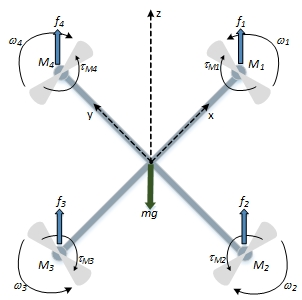
\includegraphics[width = 0.3\textwidth]{VAPIQ-PICTURES/MMFPQ.jpg}
    \caption{Quadrotor fixed pitch reference frame and forces}
    \label{fig:quadDynamics}
\end{figure}
\noindent
Fig. \ref{fig:quadDynamics} shows the quadrotor body frame of reference, "f" represents the lift force produced by the motor propeller combination. $\tau$ represents the torque and $\omega$ represents the rotational speed in rad/s.
\\\\
With these definitions in place, the rotational coordinate system can be defined. Fig. \ref{fig:quadAngles} shows the rotational angles around the body reference frame. The angle around the x axis is called roll $\phi$, the angle around the y axis is called pitch $\theta$ and last the angle around the z axis is called yaw $\psi$.
\\\\
\begin{figure}[H]
    \centering
    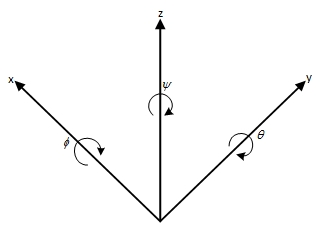
\includegraphics[width = 0.3\textwidth]{VAPIQ-PICTURES/RPJ.jpg}
    \caption{Rotational angles around the body frame}
    \label{fig:quadAngles}
\end{figure}
\\\\
 
\subsubsection{Translational Motion}

To begin with, all the movement will be along the z-axis. If the origin is placed on the ground, the z-axis value will be the altitude of the quadrotor above zero. In this section, the mathematical model from \cite{charlesdarwinuni} is used. 
\\\\
In Fig. \ref{fig:quadDynamics} you can see the 4 forces and torques acting on the quadrotor and the gravitational force \textbf{(mg)} acting in the negative z-direction. If the quadrotor is at rest and the force is grater than the weight of the quadrotor, acceleration will occur. 
\begin{equation}
  f_{tot} = f_1 + f_2 + f_3 + f_4 - mg
\end{equation}
\\
From this equation the acceleration generated by the forces acting can be obtained 
\\
\begin{equation}
  f_{tot} = ma
\end{equation}
\\
In this equation, \textbf{m} is the mass of the quadrotor \textbf{kg} and \textbf{a} is the acceleration \textbf{$m/s^2$} .
\\\\
When the motors of the quadrotor gives the same amount of force, the quadrotor will move along the z-axis. For movement along the other axes, the force on one or more of the motors must be changed. The equations of motion are
\\
\begin{equation}
f_x = f_{tot}sin\theta
\end{equation}
\begin{equation}
f_y = f_{tot}sin\phi
\end{equation}
\begin{equation}
f_z = f_{tot}cos\theta cos\phi
\end{equation}
\\
From this the acceleration can be found by substituting
\\
\begin{equation}
a_x = \frac{f_{tot}sin\theta}{m}
\end{equation}
\begin{equation}
a_y = \frac{f_{tot}sin\phi}{m}
\end{equation}
\begin{equation}
a_z = \frac{f_{tot}sin\theta cos\phi}{m}
\end{equation}
\\
By integrating the acceleration, the velocity is obtained
\begin{equation}
v_x = \int a_xdt
\end{equation}
\begin{equation}
v_y = \int a_ydt
\end{equation}
\begin{equation}
v_z = \int a_zdt
\end{equation}
\\
And by integrating the velocity, the displacement
\begin{equation}
s_x = \int v_xdt
\end{equation}
\begin{equation}
s_y = \int v_ydt
\end{equation}
\begin{equation}
s_z = \int v_zdt
\end{equation}
\clearpage

\subsubsection{Rotational Motion}
Rotational motion in space is described by rotation around three axes. For rotational motion to occur, there must be an imbalance of forces applied to the quadrotor. Rotational motion can occur in many different ways, as shown in Table \ref{tabular:rotmot}. The table shows the different force imbalances and the resulting quadrotor motion. In this section, the mathematical model from \cite{charlesdarwinuni} is used. \\\\

\begin{table}[h]
\centering
\caption{Rotational Motion}

\begin{tabular}{ |c|c|c|c| } 
 \hline \rowcolor{white}
 \textbf{Imbalance of forces} & \textbf{Roll} & \textbf{Pitch} & \textbf{Yaw} \\
 \hline
 None & - & - & - \\ 
 Opposite motors both increased & - & - & Positive/Negative \\ 
 Odd motors varied by opposite but equal amount & Positive/Negative & - & - \\ 
 Even motors varied by opposite but equal amount & - & Positive/Negative & - \\ 
 Adjacent motors both increased by the same amount & Positive/Negative & Positive/Negative & - \\ 
 All motors at unequal amount & Positive/Negative & Positive/Negative & Positive/Negative \\ 
 \hline
\end{tabular}
\label{tabular:rotmot}
\end{table} \\
\noindent
From Table \ref{tabular:rotmot} you can see that yaw motion only occurs when there is an imbalance between diagonal motor pairs. The reason for this is that the yaw motion occurs when the net torque of the motor pairs are nonzero. If these torques do not cancel out, there is a resultant torque that causes rotation about the z-axis. 
\begin{equation}
\tau_{tot} = \tau_1 + \tau_2 + \tau_3 + \tau_4
\end{equation}
\\
$\tau_{tot}$ is the resultant torque and $\tau_i$ is the torque caused by propeller $i$. Torque is measured in \textbf{Nm}. As the propeller rotates through the air, it causes drag that produces torque that is opposite to the propeller rotation. 
\begin{equation}
f_i = k\omega_i^2
\end{equation}
\begin{equation}
\tau_i = b\omega_i^2 + I_M\dot{\omega}_i
\end{equation}
\\
Where $f$ is the thrust, $k$ is the lift constant, $\tau_i$ is the torque produced by the drag force, b is the drag constant, $\omega$ is the angular velocity of the propeller, $\dot{\omega}$ is the angular acceleration and $I_M$ is the moment of inertia. 
\\\\
From these two equations it is clear that when the propellers are rotating at a constant velocity, the thrust and torque are proportional to the square of the angular velocity of the propellers. The moment of inertia contribution will be zero when the propeller is at a constant angular velocity. 
\\\\
When the conditions for yaw are met
\begin{equation}
\tau_{yaw} = \tau_{tot}\cdot l
\end{equation}
\\
Where $\tau_{yaw}$ is the torque in the yaw plane \textbf{(Nm) }and $l$ is the distance from the center of the motor to the center of the body \textbf{(m)}. This torque will produce an angular acceleration in the yaw plane. 
\begin{equation}
\tau_{yaw} = a_{yaw}\cdot I_{zz}
\end{equation}
\\
Where $a_{yaw}$ is the angular acceleration in $rad/s^2$ in the yaw plane and $I_{zz}$ is the moment of inertia in the yaw or $zz$ plane in $kg.m^2$. Substituting equation (19) with (15) and (18) we get the angular acceleration
\begin{equation}
a_{yaw} = \frac{(\tau_1 + \tau_2 + \tau_3 + \tau_4) \cdot l}{I_{zz}}
\end{equation}
\\ 
Since all of these variables are known or can be calculated, the acceleration in the yaw plane can be determined. 
\\\\
The torque can also be manipulated to produce roll motion in the xz-plane. For roll motion there has to be an unbalance between the left and right hand side, or other combinations, as seen in Table \ref{tabular:rotmot}. 
\begin{equation}
f_{roll} = f_2 - f_4
\end{equation}
\\
Where $F_{roll}$ is the resultant force in \textbf{Nm} in the roll direction. This will cause the quadrotor to have roll motion. 
\begin{equation}
\tau_{roll} = f_{roll}\cdot l
\end{equation}
\\
Where $\tau_{roll}$ is the resultant torque in \textbf{N} in the roll direction. Substituting the same way as for yaw, gives
\begin{equation}
a_{roll} = \frac{\tau_{roll}}{I_{yy}}
\end{equation}
\\
Where $a_{roll}$ is the angular acceleration in $rad/s^2$ in the roll plane, and $I_{yy}$ is the moment of inertia in the roll or $yy$ plane in $kg.m^2$. 
\\\\
Substituting equation (16) into equation (23) gives the expression for angular acceleration proportional to the motor speed
\begin{equation}
a_{roll} = \frac{(k\omega_2^2-k\omega_4^2)\cdot l}{I_{yy}}
\end{equation}
\\\\
Since the same logic applies to pitch movement the expression for acceleration in the pitch plane can be obtained from equation (24). 
\begin{equation}
a_{pitch} = \frac{(k\omega_1^2-k\omega_3^2)\cdot l}{I_{xx}}
\end{equation}
\\
Where $a_{pitch}$ is the angular acceleration in $rad/s^2$ in the pitch plane and $I_{xx}$ is the moment of inertia in the pitch or $xx$ plane in $kg.m^2$. 
\\\\
Since the quadrotor is operating in discrete time, expressions for angular velocity and angular displacement in the roll, pitch and yaw directions can be found 
\begin{equation}
\omega_{roll} = (a_{roll} - a_{roll-1})ts
\end{equation}
\begin{equation}
\omega_{pitch} = (a_{pitch} - a_{pitch-1})ts
\end{equation}
\begin{equation}
\omega_{yaw} = (a_{yaw} - a_{yaw-1})ts
\end{equation}
\\
\begin{equation}
\theta = (\omega_{roll} - \omega_{roll-1})ts
\end{equation}
\begin{equation}
\phi = (\omega_{pitch} - \omega_{pitch-1})ts
\end{equation}
\begin{equation}
\psi = (\omega_{yaw} - \omega_{yaw-1})ts
\end{equation}
\\
Where $\omega_{roll}$, $\omega_{pitch}$ and $\omega_{yaw}$ are the angular velocities in $rad/s$ in the roll, pitch and yaw directions, and $\theta$, $\phi$ and $\psi$ are the angular displacement in $rad$ in the roll, pitch and yaw directions.  
\begin{comment}
\subsection{Quaternions FPQ}
To be able to combine both translational motion and rotational motion, an often used approach must be implemented. This approach is called The Newton-Euler equations. This model allows us to describe the combination of translational motion and rotational motion of a rigid body. 
\\\\
This way of modeling is considered a fundamental approach, but it still has three drawbacks \cite{lule}. 
\begin{enumerate}
    \item First of all it is exclusively based on Euler angles, which have the trait of being intuitive, but per definition these angles can not define certain orientations because it suffers from singularities that leads to a problem known as "gimbal lock" \cite{gimbal}. Gimbal lock is the loss of one degree of freedom in a three-dimensional space, that occurs when the axes of two of the three rotational axes are driven into a parallel configuration, "locking" the system into rotation in a degenerate two-dimensional space. 
    \item The second drawback is that it is very computationally expensive. To calculate sines and cosines takes a lot of performance and can become unmanageable, especially if it is being implemented on low-cost hardware. 
    \item The last drawback is that when creating estimators or controllers it is necessary to add the Jacobian of the system states. This makes the computational cost even greater, because all the matrix elements will have one or more sines or cosines to compute. This can quickly overwhelm the system. 
\end{enumerate}
\\\\
To overcome these three drawbacks there are three solutions: 
\begin{enumerate}
    \item To guarantee that the system will be kept inside the bounds of Euler angles. \\
    - If the quadrotor only will be used for simple and stable flight, this method might work, but you always have to consider unknown external disturbance such as wind turbulence, which can result in flipping the quadrotor. Therefore this approach will not be able to compensate for the drawbacks. 
    \item To utilize a Direction Cosine Matrix (DCM) approach.\\
    - For this approach, a DCM is constructed by translating the x, y and z coordinate system into a $3x3$ matrix. No matter how you rotate this coordinate system, the matrix will still represent this transformation. The most significant merit of this approach is the non-suffering from the singularities, as the Euler angles do. There is still a downside to this approach. The DCM suffers from the constraint that each axis must be orthogonal to the other axes and should also be of a unit length. When you are rotating a DCM you must multiply it with another DCM. The derivative of the DCM results in a $3x3$ matrix, which is implemented into a system of nine coupled differential equations to be solved. You can get away with calculating only six coupled differential equations if the third axis is calculated from the cross product of the other two. 
    \item To implement the quaternion approach. \\
    - In the last approach the previous mentioned drawbacks or limitations do not exist. You can directly translate a quaternion into a DCM and translate a DCM into a quaternion. However this approach has a constraint. The quaternion and its corresponding derivative has four values and the constraint is that it must be of unit length. This means that we have a system of four coupled differential equations, greatly decreasing the computational cost and keeping the overall complexity low. Since quaternions are complex numbers it can be hard to understand what it represents, but the direct coupling to a DCM makes the translation easy. 
\end{enumerate}

\subsubsection{Quaternion Algebra}
This section describes quaternion based modeling \cite{lule}. Quaternions is a complex number similar to ordinary complex numbers. A complex number is described as  a +  bi, where a and b are real numbers, and i is the imaginary unit i.e a,b $\in$ $\mathbb{R}$ and $i^2$ = -1.
\begin{figure}[H]
    \centering
    \includegraphics[width = 0.3\textwidth]{VAPIQ-PICTURES/ComplexUnitCire.gif}
    \caption{PICTURE caption}
    \label{fig:unitCircle}
\end{figure}
\noindent
An extension of this system leads to the quaternions. Quaternions is used to calculate three dimensional rotations, therefore they are useful in describing flight. Quaternions are denoted as
\begin{equation}
q = q_0 + q_1i + q_2j + q_3k
\end{equation}
where $q_1$, $q_2$, $q_3$ is the vector part, and $q_o$ is a scalar. Note that describing 3 dimensional rotation requires 4 dimensions.% is this correct?
\begin{equation}
q = \begin{bmatrix}
    q_0 & q_1 & q_2 & q_3 
\end{bmatrix}^T
\end{equation}
The inverse of a quaternion has the same definition as ordinary complex numbers, switch the sign of the complex part.
\begin{equation}
Conj(\textbf{q}) = \textbf{q}^* = \begin{bmatrix}
    q_0 & -q_1 & -q_2 & -q_3 
\end{bmatrix}^T
\end{equation}
An important feature of quaternions is that multiplication is non-commutative. i.e
\begin{equation}
    p\cdot q \neq q\cdot q
\end{equation}
So the multiplication order matters. Ordinary complex numbers on the other hand is commutative.
The general rule for multiplication between the quaternions are
\begin{equation}
i^2 = j^2 = k^2 = ijk = -1
\end{equation}
The following table summarizes multiplication rules applied to quaternions.
\begin{table}[h]
\centering
\begin{tabular}{ |c|c|c|c| }
 \hline
 \textbf{} & \textbf{i} & \textbf{j} & \textbf{k} \\ 
 \hline
\textbf{i} & -1 & k & -j \\
\textbf{j} & -k & -1 & i \\
\textbf{k} & j & -i & -1 \\ 
\hline
\end{tabular}
\caption{Multiplication rules}
\label{tabular:quatRules}
\end{table}
\\
Lets denote p =
\begin{bmatrix}
    p_0 & p_1 & p_2 & p_3 
\end{bmatrix}$^T$,
and q = \begin{bmatrix}
    q_0 & q_1 & q_2 & q_3 
\end{bmatrix}$^T$.  If p and q represents two individual rotations, the Kroenecker product $p\otimes q$ represents the combined rotation. By using the multiplication rules and equation (32), the following matrices are obtained.
\begin{equation}
p\otimes q=
\begin{bmatrix}
p_oq_o - p_1q_1 - p_2q_2 - p_3q_3 \\
p_0q_1 + p_1q_0 + p_2q_3 - p_3q_2\\
p_0q_2 - p_1q_3 + p_2q_0 + p_3q_1\\
p_0q_3 + p_1q_2 - p_2q_1 + p_3q_0
\end{bmatrix}
\end{equation}
\\ 
\begin{equation}
= Q(p)q = 
\begin{bmatrix}
p_o & -p_1 & -p_2 & -p_3 \\
p_1 & p_0 & -p_3 & p_2\\
p_2 & p_3 & p_0 & -p_1\\
p_3 & -p_2 & p_1 & p_0
\end{bmatrix}
\begin{bmatrix}
q_0\\
q_1\\
q_2\\
q_3
\end{bmatrix}
\end{equation}
\\
\begin{equation}
= \bar{Q}(q)p = 
\begin{bmatrix}
q_o & -q_1 & -q_2 & -q_3 \\
q_1 & q_0 & -q_3 & -q_2\\
q_2 & -q_3 & q_0 & q_1\\
q_3 & q_2 & -q_1 & q_0
\end{bmatrix}
\begin{bmatrix}
p_0\\
p_1\\
p_2\\
p_3
\end{bmatrix}
\end{equation}
The magnitude of a quaternion is defined as
\begin{equation}
  Norm(q) = \|q\| = \sqrt{q_0^2 + q_1^2 + q_2^2 + q_3^2}
\end{equation}
\\
As you can see from equation (40), the magnitude (norm) of a quaternion is defined in the same way as the magnitude of a vector. In this approach, all% only this approach??
quaternions are assumed to be of unit length and are therefore called unit quaternions.
\\\\
The same applies for the inverse of a quaternion, it is the same rule for the inverse of a quaternion as the inverse of a normal complex number. However, if the length of the quaternion is unit, then the inverse is the same as the conjugate.
\\
\begin{equation}
  Inv(q) = q^{-1} = \frac{q*}{\|q\|^2}
\end{equation}
The derivative of the quaternion in the fixed frame is
\begin{equation}
   \dot{\textbf{q}}_\omega(\textbf{q}, \omega) = \frac{1}{2} \textbf{q} \otimes \begin{bmatrix}
    0 \\[0.3em]
    \omega\\[0.3em]
\end{bmatrix} = \frac{1}{2} Q(\textbf{q}) \begin{bmatrix}
    0 \\[0.3em]
    \omega\\[0.3em]
\end{bmatrix}
\end{equation}
while the derivative of the quaternion in the body frame is
\begin{equation}
   \dot{\textbf{q}}_\omega\prime(\textbf{q}, \omega\prime) = \frac{1}{2} \begin{bmatrix}
    0 \\[0.3em]
    \omega\prime\\[0.3em]
\end{bmatrix} \otimes \textbf{q} = \frac{1}{2} \overline{Q}(\textbf{q}) \begin{bmatrix}
    0 \\[0.3em]
    \omega\prime\\[0.3em]
\end{bmatrix}
\end{equation}
where
\begin{equation}
\omega = 
\begin{bmatrix}
    \omega_x &\omega_y & \omega_z
\end{bmatrix}^T
\end{equation}
If the quaternion is a unit quaternion, it can be used to describe rotation. The following equation rotates a vector \textbf{v} from the fixed frame to the body frame.
\begin{equation}
  \omega = \textbf{q} \otimes \begin{bmatrix}
    0 \\[0.3em]
    \textbf{v}\\[0.3em]
\end{bmatrix} \otimes \textbf{q}^*
\end{equation}
Equation (45) can also be described with respect to the x , y and z axis.
\begin{equation}
  R_x(\textbf{q}) = \textbf{q} \otimes \begin{bmatrix}
    0 \\[0.3em]
    1\\[0.3em]
    0 \\[0.3em]
    0\\[0.3em]
\end{bmatrix} \otimes \textbf{q}^* = \begin{bmatrix}
    q_0^2 + q_1^2 - q_2^2 - q_3^2 \\[0.3em]
    2(q_1q_2 + q_0q_3)\\[0.3em]
    2(q_1q_3 - q_0q_2) \\[0.3em]
\end{bmatrix}
\end{equation}
\begin{equation}
  R_y(\textbf{q}) = \textbf{q} \otimes \begin{bmatrix}
    0 \\[0.3em]
    0\\[0.3em]
    1 \\[0.3em]
    0\\[0.3em]
\end{bmatrix} \otimes \textbf{q}^* = \begin{bmatrix}
    2(q_1q_2 - q_0q_3)\\[0.3em]
    q_0^2 - q_1^2 + q_2^2 - q_3^2 \\[0.3em]
    2(q_2q_3 + q_0q_1) \\[0.3em]
\end{bmatrix}
\end{equation}
\begin{equation}
  R_z(\textbf{q}) = \textbf{q} \otimes \begin{bmatrix}
    0 \\[0.3em]
    0\\[0.3em]
    0 \\[0.3em]
    1\\[0.3em]
\end{bmatrix} \otimes \textbf{q}^* = \begin{bmatrix}
    2(q_1q_3 + q_0q_2)\\[0.3em]
    2(q_2q_3 - q_0q_1) \\[0.3em]
    q_0^2 - q_1^2 - q_2^2 + q_3^2 \\[0.3em]
\end{bmatrix}
\end{equation}
The total rotation matrix is denoted 
R(\textbf{q}) = \begin{bmatrix}
 R_x(\textbf{q})^T\\[0.3em]
    R_y(\textbf{q})^T \\[0.3em]
    R_z(\textbf{q})^T \\[0.3em]
\end{bmatrix}
\subsubsection{Conversion from Euler Angles to Quaternions}
%The angles α, β and γ are uniquely determined except for the singular case that the xy and the XY planes are identical, i.e. when the z axis and the Z axis have the same or opposite directions. Indeed, if the z axis and the Z axis are the same, β = 0 and only (α + γ) is uniquely defined (not the individual values), and, similarly, if the z axis and the Z axis are opposite, β = π and only (α − γ) is uniquely defined (not the individual values). These ambiguities are known as gimbal lock in applications
Euler angles are defined for all angles except for when the body frame and the frame of reference has identical xy planes, this case is called a singularity and the Euler angle is not defined. To be able to describe this scenario the Euler angles needs to be converted into quaternions. The following two equations can be used to convert from Euler angles to quaternions.
\begin{equation}
  \textbf{q} = \begin{bmatrix}
    \cos(\frac{\phi}{2})\cos(\frac{\theta}{2})\cos(\frac{\psi}{2})+\sin(\frac{\phi}{2})\sin(\frac{\theta}{2})\sin(\frac{\psi}{2})\\[0.3em]
    
    \sin(\frac{\phi}{2})\cos(\frac{\theta}{2})\cos(\frac{\psi}{2})-\cos(\frac{\phi}{2})\sin(\frac{\theta}{2})\sin(\frac{\psi}{2})\\[0.3em]
    
    \cos(\frac{\phi}{2})\sin(\frac{\theta}{2})\cos(\frac{\psi}{2})+\sin(\frac{\phi}{2})\cos(\frac{\theta}{2})\sin(\frac{\psi}{2})\\[0.3em]
    
    \cos(\frac{\phi}{2})\cos(\frac{\theta}{2})\sin(\frac{\psi}{2})-\sin(\frac{\phi}{2})\sin(\frac{\theta}{2})\cos(\frac{\psi}{2})\\[0.3em]
\end{bmatrix}
\end{equation}
where
\begin{equation}
 \begin{bmatrix}
    \phi   \\[0.3em]
    \theta \\[0.3em]
    \psi   \\[0.3em]
\end{bmatrix} = \begin{bmatrix}
    atan2(2(q_0q_1 + q2_q3)), q_0^2 - q_1^2 - q_2^2 + q_3^2\\[0.3em]
    asin(2(q_0q_2-q_3q_1))\\[0.3em]
    atan2(2(q_0q_3 + q_1q_2)), q_0^2+ q_1^2-q_2^2q_3^2
\end{bmatrix}
\end{equation}
\subsubsection{Quaternion based Modeling FPQ}
To model the attitude dynamics of a quadrotor, it is necessary to assume that the structure is rigid and symmetrical. It is also necessary to assume that only the differential forces created by the four propellers have an effect on the rotation.
\\\\
When modeling the physics of a quadrotor, two alternative approaches can be followed \cite{lule}. 
\begin{enumerate}
    \item To make a full physical model that will be derived from the utilization of Newtons´ laws of motion and to make a frame dependent model. % Make clearer
    \item To use the Euler-Newton equations for the combination of translational and rotational motion of a rigid body. 
\end{enumerate}
\\
The second approach will simplify the derivation of the model because the only unknown part of this model is the connection from the control signal and the corresponding torque \cite{newtoneuler}. \\\\
\begin{equation}
\begin{bmatrix}
    F \\[0.3em]
    \tau\\[0.3em]
\end{bmatrix}
=
\begin{bmatrix}
    m & 0 \\[0.3em]
    0 & I_{cm}\\[0.3em]
\end{bmatrix}
\begin{bmatrix}
    a_{cm} \\[0.3em]
    \dot{\omega}\\[0.3em]
\end{bmatrix}
+ 
\begin{bmatrix}
    0 \\[0.3em]
    \omega\times(I_{cm}\cdot\omega)\\[0.3em]
\end{bmatrix}
\end{equation}
Where $\omega$ is defined as 
\begin{equation}
\omega = 
\begin{bmatrix}
    \omega_x \\[0.3em]
    \omega_y\\[0.3em]
    \omega_z
\end{bmatrix}
\end{equation}\\
and $F$ is the total force acting on the centre of the mass, $m$ is the mass of the body, $I_{cm}$ is the moment of inertia about the centre of the mass, $a_{cm}$ is the acceleration of the centre of the mass, $\dot{\omega}$ is the angular acceleration of the body and $\omega$ is the angular velocity of the body. 
\\\\
To derive a description of the full dynamics of the quadrotors rigid body rotations, equation (43) should be combined with the rotation dynamics from equation (51). This results in an equation system describing the whole rotation dynamics of the quadrotor. This equation system is described using the quaternion approach. 
\begin{equation}
  \begin{cases}
    \dot{q} = - \frac{1}{2}\begin{bmatrix}
    0 \\[0.3em]
    \omega\\[0.3em]
    \end{bmatrix}\bigotimes q\\
        \dot{\omega} = I_{cm}^{-1}\cdot\tau-I_{cm}^{-1}
    \begin{bmatrix}
    \omega \times (I_{cm}\cdot \omega)\\[0.3em]
    \end{bmatrix}
  \end{cases}
\end{equation}\\

%This description of the entire rotation of the quadrotor is used in our controller. 
\end{comment}

\newpage
\subsection{Variable Pitch Quadcopter}

A variable pitch quadcopter has six degrees of freedom. $\phi$, $\theta$ and $\psi$ represents roll, pitch and yaw angles. $v_x$,$v_y$ and $v_z$ represents the flight velocities in the body frame. The force $f$ generated by the propellers and motors is given by
\begin{equation}
    f_{i} = k\alpha_i\omega_i^2
\end{equation}
Where $k$ is the aerodynamic constant,  $\alpha$ is the propeller pitch angle. and $\omega$ is the rotational speed of the propeller. Comparing this equation to equation (16), it can be seen that the only difference is the pitch blade angle $\alpha$.
\begin{figure}[H]
    \centering
    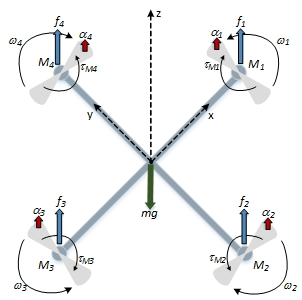
\includegraphics[width = 0.3\textwidth]{VAPIQ-PICTURES/MMVPQ.jpg}
    \caption{Variable Pitch Quadrotor, Frame Of Reference And Forces}
    \label{fig:ControllInputs}
\end{figure}
\noindent
Figure \ref{fig:ControllInputs} shows the axes along with the lift force and torque vectors, pitch angle $\alpha$ and the rotational speed $\omega$. The total lift force in the z-axis generated by the motors and propellers is given by
\begin{equation}
   f_{z} = \sum_{i=1}^{4} f_{i} = \sum_{i=1}^{4} k\alpha_i\omega_i^2
\end{equation}
The drag produced by the motor and propeller can be approximated by the equation
\begin{equation}
   Q_j = b_{D1}\alpha_j^2\omega_j^2 + b_D_2\omega_j^2 + b_{D3}\alpha_j\omega_j
\end{equation}
Where $b_{D1}$,$b_{D1}$ and $b_{D1}$ is aerodynamical constants. The torques used to control roll, pitch and yaw moments can be described by the following equations.
\begin{equation}
   \tau_\phi = l(L_2-L_4) =lk(\alpha_2\omega_2^2-\alpha_4\omega_4^2)
\end{equation}
\begin{equation}
   \tau_\theta = l(L_3-L_1) = lk(\alpha_3\omega_3^2-\alpha_1\omega_1^2)
\end{equation}
\begin{equation}
   \tau_\psi = Q_1 + Q_3 - Q_4 - Q_2
\end{equation}
Where l is the distance from the propellers center to center of gravity of the quadcopter.
\\\\
Comparing the variable pitch quadrotor equations for roll, pitch and yaw with the fixed pitch equations for roll, pitch and yaw, it can be seen that the only difference is the propeller pitch angle $\alpha$. This shows that the controller logic is quite similar for the variable pitch quadrotor as for the fixed pitch quadrotor.
\newpage
%%%%%%%%%%%%%%%%%%%%%%%%%%%%%%%%%%%%%%%%%%%%%%%%%
%%%%%%%%%%%%%%%%%%%%%%%%%%%%%%%%%%%%%%%%%%%%%%%%%

\subsection{Motor Model}
The following motor model is derived based on the motor model described in the report from MIT \cite{MITvpp}. The motor model presented is a simplified representation of a three phase motor described as a basic DC motor. %En antagelse/forenkling gjør at vi bruker denne.
\\\\
In order to make the motor model, different motor constants for the specific motors used in this project needs to be determined. These constants can be found in the datasheet \cite{AXI}, and are given in Tab. \ref{tab:motconst}.

\begin{table}[H]
\centering
\caption{Motor Constants}
\label{tab:motconst}
\begin{tabular}{ |c|c| } 
 \hline
 $K_v$ [rad/s/v] & 148.702 \\ 
 \hline
 R [$\Omega$] & 0.155 \\ 
 \hline
 $i_0$ [A] & 0.6 \\ 
 \hline
\end{tabular}
\end{table}
\noindent
A basic DC motor is modeled as a circuit with a voltage source in series with a resistor and an inductor. By applying Kirchhoff's laws, equation (38) is obtained. 

\begin{equation}
    v = Ri + L\frac{\partial i}{\partial t} + e
\end{equation} 
Where $R$ is the internal motor resistance, $i$ is the current, $L$ is the motor inductance and $e$ is the back EMF. The back EMF, $e$, can be described as
\begin{equation}
    e = \frac{\omega}{K_v}
\end{equation}
where $\omega$ is the rotational speed [rad/s] and $K_v$ is the voltage constant of the motor [rad/s/v]. The motor model can then be rewritten as
\begin{equation}
    v = Ri + L\frac{\partial i}{\partial t} + \frac{\omega}{K_v}
\end{equation}
\\\\
The motor torque $\tau_M$ can be modeled as proportional to the difference between the current, $i$, and the no-load current, $i_0$, divided by the torque constant, $K_Q$.  
\begin{equation}
    \tau_M = \frac{i - i_0}{K_Q}
\end{equation}
\\\\
The motor dynamics can be modeled as a first order differential equation
\begin{equation}
    I\dot{\omega} = \tau_M - \tau_L
\end{equation}
where $\tau_M$ represents the motor torque produced by the voltage source, the load torque, $\tau_L$, is produced by the propeller drag and $I$ is the moment of inertia of the rotating parts. 
\\\\
When using small brushless motors, the inductance is typically very small compared to the physical response of the system and can be neglected \cite{MITvpp}. When neglecting the inductance, substituting equation (40) and (41) into equation (42) yields the following equation for $\dot\omega$.

\begin{equation}
    I\dot{\omega} =\left[\left(u-\frac{\omega}{K_v}\right)\frac{1}{R}-i_0\right]\frac{1}{K_Q} - \tau_L
\end{equation}
\newpage

\subsection{Motor-Propeller Model}
\subsubsection{Non Linear Motor-Propeller Model}

\begin{equation}
    L = \rho cR_p^3\omega^2C_{L\alpha}\frac{\alpha}{3}
\end{equation}

\begin{equation}
    \tau_L =  \rho cR_p^4\omega^2\left(\frac{C_{D0} + C_{Di}\alpha^2}{4} - \frac{C_{L\alpha}\alpha\omega}{3R_p}\right)
\end{equation}
\\\\
These two equations shows the lift $L$ and drag $T_L$ produced by the motor-propeller combination. From these two equations it is shown that the lift and the drag is affected by the motor speed $\omega$ and the propeller pitch angle $\alpha$. The remaining terms of the equations are constants. This shows that to change the lift, you have to change either the pitch angle $\alpha$ or the motor speed $\omega$. By changing and combining the remaining constants of equations (44) and (45), equations (46) and (47) can be obtained. 

\begin{equation}
    L = b_L\omega^2\alpha
\end{equation}

\begin{equation}
    \tau_L = b_{D_1}\omega^2 + b_{D_2}\omega^2\alpha^2 + b_{D_3}\omega\alpha
\end{equation}
\\\\
Where $b_L$, $b_{D1}$, $b_{D1}$ and $b_{D1}$ are estimated lift and drag coefficients. These coefficients are obtained from the Variable Pitch Quadcopter report from MIT \cite{MITvpp} using the same propellers. The coefficients were selected by first identifying a similar symmetrical, tapered propeller in the NACA(National Advisory Committee for Aeronautics) database of airfoils. The particular airfoil chosen was the NACA 009. Using software the coefficients Tab. \ref{tab:EsLiDrCo} were estimated by MIT.

\begin{table}[H]
\caption{Estimated Lift and Drag coefficients}
\label{tab:EsLiDrCo}
\centering
\begin{tabular}{ c c c c} 
 \hline
 b_L & b_{D1} & b_{D2} & b_{D3}\\
 3.88e-07 & 9.96e-09 & 2.46e-10 & 4.33e-07 \\
 \hline
\end{tabular}
\end{table}

Substituting equation (47) into equation (43) yields the following equation.

\begin{equation}
    I\dot{\omega} = \left[ \left(v - \frac{\omega}{K_v}\right) \frac{1}{R} - i_0 \right]\frac{1}{K_Q} - b_{D_1}\omega^2 - b_{D_2}\omega^2\alpha^2-b_{D3}\omega\alpha
\end{equation}
\\\\
This equation is the nonlinear differential equation for $\dot\omega$.

%%%%%%%%%%%%%%%%%%%%%%%%%%%%%%%%%%%%%%%%%%%%%%%%%
%%%%%%%%%%%%%%%%%%%%%%%%%%%%%%%%%%%%%%%%%%%%%%%%%

\newpage

\subsubsection{Linearized Motor-Propeller Model}

To develop further insights into the dynamics of the motor, such as response time and steady state values, equation (48) needs to be linearized. The nonlinear equation (48) can be linearized at near hover conditions, using $\omega_0$ and $\alpha_0$. $\omega_0$ and $\alpha_0$ is the start rotational speed and pitch angle at hover, there are a infinite number of possible combinations of these that will yield hover. The linearization used is taken from the report from MIT \cite{MITvpp}. This yields equation (49) and (50) which is the resulting state-space system. 

\begin{equation}
    \Delta\dot{\omega} = \left[-\frac{1}{RK_VK_QI}-\frac{2b_D_1\omega_0}{I}-\frac{2b_D_2\omega_0\alpha_0^2}{I}-\frac{b_3\alpha_0}{I}\right]\Delta\omega + \left[\frac{1}{RK_QI}\quad - \frac{2b_D_2\omega_0^2\alpha_0}{I} + \frac{b_d3\omega_0}{I}  \right] \begin{bmatrix}
       \Delta v            \\[0.2em]
       \Delta\alpha \\[0.2em]
     \end{bmatrix}
\end{equation}

\begin{equation}
    \Delta L = \left[2b_L\omega_0\alpha_0 \right]\Delta\omega + \left[0\quad b_L\omega_0^2\right]
    \begin{bmatrix}
        \Delta v \\
        \Delta\alpha
    \end{bmatrix}
\end{equation}

Solving the multiplications of the matrices, equations (51) and (52) are obtained. 

\begin{equation}
    \Delta\dot{\omega} = \left(-\frac{1}{RK_VK_QI}-\frac{2b_D_1\omega_0}{I}-\frac{2b_D_2\omega_0\alpha_0^2}{I}-\frac{b_{D3}\alpha_0}{I}\right)\Delta\omega + \frac{1}{RK_QI}\Delta v - \left(\frac{2b_D_2\omega_0^2\alpha_0}{I} - \frac{b_{D3}\omega_0}{I}\right)\Delta\alpha
\end{equation}

\begin{equation}
    \Delta L = 2b_L\omega_0\alpha_0\Delta\omega + b_L\omega_0^2\Delta\alpha
\end{equation}

This system has two inputs and one output, which makes it a MISO system (Multiple Input, Single Output). The two inputs are the change in applied motor voltage, $\Delta v$, and change in propeller pitch/angle, $\Delta\alpha$. The output of the system is the change in lift, $\Delta L$, produced by the propellers. Based on equation (49) and (50), a state-space canonical form block diagram can be created. Fig. \ref{fig:canonical} shows this block diagram. 

\begin{figure}[H]
    \centering
    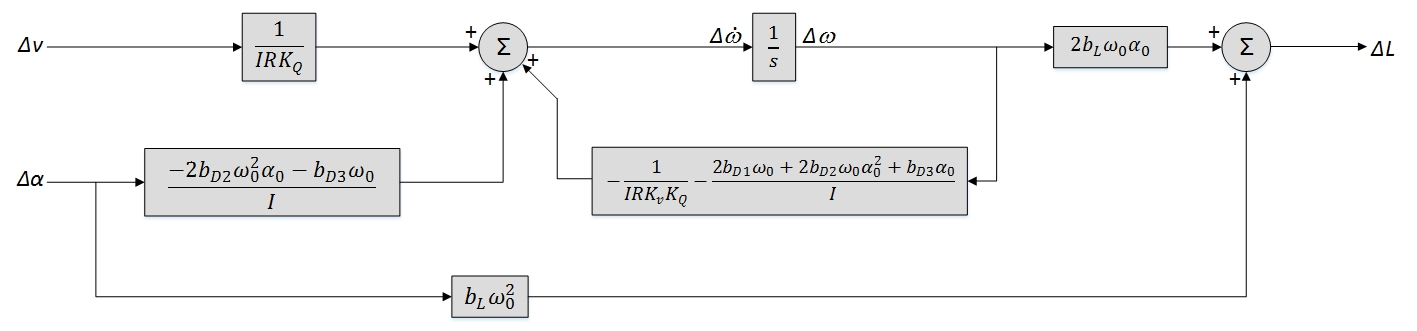
\includegraphics[width = 1\textwidth]{VAPIQ-PICTURES/canonicalblock.jpg}
    \caption{State-Space Canonical Block Diagram}
    \label{fig:canonical}
\end{figure}

\begin{equation}
    \dot x = Ax + Bu
\end{equation}

\begin{equation}
    y = Cx + Du
\end{equation}

Equation (53) and (54) shows a traditional representation of a state-space system. As seen from equation (49) and (50), this is the state-space representation of the motor-propeller model, where $\Delta\dot\omega = \dot x$, $\Delta\omega = x$, $\Delta L = y$ and     \begin{bmatrix}
        \Delta v \\
        \Delta\alpha
    \end{bmatrix} $=u$. 

\begin{equation}
    A = \left[-\frac{1}{RK_VK_QI}-\frac{2b_D_1\omega_0}{I}-\frac{2b_D_2\omega_0\alpha_0^2}{I}-\frac{b_{D3}\alpha_0}{I}\right]
\end{equation}

\begin{equation}
    B = \left[\frac{1}{RK_QI}\quad - \frac{2b_D_2\omega_0^2\alpha_0}{I} - \frac{b_{D3}\omega_0}{I}  \right]
\end{equation}

\begin{equation}
    C = \left[2b_L\omega_0\alpha_0 \right]
\end{equation}

\begin{equation}
    D = \left[0\quad b_L\omega_0^2\right]
\end{equation}

Equation (49) and (50) also yields A, B, C and D matrices for the state-space model. 

\begin{comment}
Simulering, 
\end{comment}